%This work is licensed under the Creative Commons License Attribution 4.0 International (CC-BY 4.0)
%https://creativecommons.org/licenses/by/4.0/legalcode
\documentclass[rgb]{standalone}
\usepackage{tkz-euclide}
\usepackage{amsmath}
\definecolor{myorange}{hsb}{0.0833, 1, 0.8}
\definecolor{mygreen}{hsb}{0.3333, 1, 0.8}
\definecolor{myblue}{hsb}{0.5833, 1, 0.8}
\definecolor{mymagenta}{hsb}{0.8333, 1, 0.8}
\begin{document}
	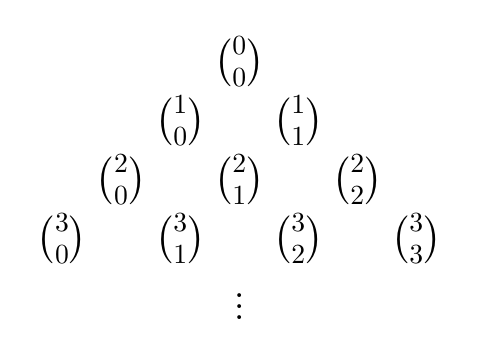
\begin{tikzpicture}[scale=1.5, font=\Large]
	\foreach \i in {0,...,3} {
		\foreach \j in {0,...,\i} {
			\draw node[anchor=center] at (1*\j-0.5*\i,-0.5*\i) {$\binom{\i}{\j}$};
		}
	}
	\draw node[anchor=center] at (0,-2) {$\vdots$};
	\end{tikzpicture}
\end{document}